
%(BEGIN_QUESTION)
% Copyright 2009, Tony R. Kuphaldt, released under the Creative Commons Attribution License (v 1.0)
% This means you may do almost anything with this work of mine, so long as you give me proper credit

A simple proportional-only pneumatic controller such as the one shown below has a serious shortcoming.  There is no way for an operator to ``manually'' take control of the process!  The controller, as built, will always be in the ``automatic'' mode of operation:

$$\includegraphics[width=15.5cm]{i01478x01.eps}$$

\filbreak

We can give this controller manual-mode capability by adding a hand pressure regulator and a ``transfer'' valve:

$$\includegraphics[width=15.5cm]{i01478x02.eps}$$

There is still a problem, though.  Imagine if you were an operator, about to switch the controller from ``Auto'' to ``Manual'' mode or vice-versa.  What problem would you encounter as you did this?

\underbar{file i01478}
%(END_QUESTION)





%(BEGIN_ANSWER)

The odds of making a smooth, ``bumpless'' transfer from one mode to the other will be very slim!

%(END_ANSWER)





%(BEGIN_NOTES)

The key to understanding the problem is to realize that the operator cannot tell if there is a difference between the hand regulator's pressure output and the controller mechanism's output before making the switch.

%INDEX% Control, proportional: bumpless output transfer (pneumatic)

%(END_NOTES)


